\chapter{Механизм поддержания продольных вихрей} \label{OXgen_ch}

При исследовании модельного порыва определены основные элементы цикла его самоподдержания. Полученные результаты согласуются с существующими представлениями о механизме поддержания организованных структур в пристенных турбулентных течениях \cite{Hamilton1995, Waleffe1995, Waleffe1997, Jimenez1999, Schoppa2002}. Основным элементом организованных структур являются полосы повышенно и пониженной скорости, наблюдающиеся в буферном слое \cite{Kline1967, Smith1983}. Полосы в турбулентном течении перемещаются вдоль стенки и имеют ограниченное время жизни, но они достаточно хорошо различимы на фоне мелкомасштабных турбулентных пульсаций. Образование пульсаций в потоке связывают с неустойчивостью сдвиговых слоев, присутствующих в полосчатом течении. В работе \cite{Kim1971} сделан вывод о том, что производство турбулентных пульсаций в пристенных течениях практически полностью обусловлено периодически повторяющимся взрывообразным развитием неустойчивости на полосах пониженной скорости (<<bursting phenomena>>). Считается, что существование полос поддерживают продольные вихри за счет <<лифт-ап>> эффекта. Детали механизма регенерации пристенных структур и, в первую очередь, механизмы образования продольных вихрей в настоящее время не установлены. Результаты исследования модельного порыва могут расширить существующие представления о механизме регенерации пристенных структур. 

В этой главе описан механизм поддержания стационарных продольных вихрей, найденный при изучении модельного порыва. Также в главе описано решение уравнений Навье-Стокса, имеющее вид трехмерной бегущей волны, и механизм поддержания продольных вихрей в этом решении. Решение, имеющее вид бегущей волны, периодично вдоль потока и стационарно в сопутствующей системе отсчета. Оно является предельным состоянием решения, эволюционирующего на сепаратрисе, найденного в непротяженной расчетной области. Имея более простую форму и поведение во времени, это решение воспроизводит механизм поддержания колебаний, аналогичный механизму поддержания колебаний в модельном порыве. Описание механизма поддержания продольных вихрей на примере решения в виде бегущей волны имеет более простой вид и позволяет более строго продемонстрировать особенности движения, обеспечивающие работу этого механизма. 

Основные результаты, представленные в главе, описаны в статьях автора диссертации \cite{MZG2017, KMU17}. 



\section{Решение в виде бегущей волны} \label{pipe_tw_seq}

Модельному порыву соответствует предельное решение на сепаратрисе, найденное в протяженной расчетной области с дополнительными условиями симметрии \eqref{sym_eq}, \eqref{per_eq}. Пульсационная составляющая движения в этом решении имеет форму бегущей волны длиной около 5 радиусов трубы $R$. В согласии с \cite{Avila2013}, предельное решение на сепаратрисе, найденное при тех же условиях, что и модельный порыв, и дополнительном условием $5R$-периодичности вдоль трубы, имеет более простую динамику, а именно, имеет вид бегущей волны, поле скорости которой стационарно в подходящей подвижной системе отсчета. Решение, имеющее вид бегущей волны, повторяет особенности бегущей волны, наблюдаемой в модельном порыве, и воспроизводит общий с модельным порывом механизм поддержания колебаний. Фазовая скорость найденной бегущей волны $c_\mathrm{tw} = 0.77$ (<<tw>> --- <<traveling wave>>) и близка к фазовой скорости бегущей волны в модельном порыве. Метод поиска решения на сепаратрисе описан в разделе \ref{edge_seq}. 

\begin{figure}
\center{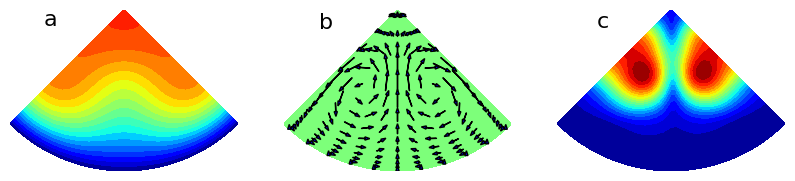
\includegraphics[width=1\linewidth]{pipetw_means.png}}
\center{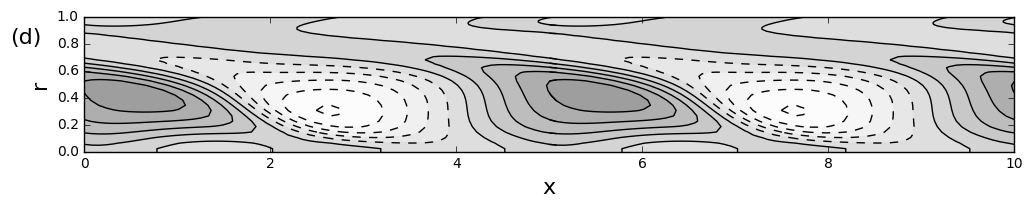
\includegraphics[width=1\linewidth]{pipetw_v1_ls.png}}
\caption{Поле скорости решения, имеющего вид бегущей волны: (a) --- изолинии продольной компоненты $\V_\mathrm{tw}$ , (b) --- векторное поле поперечной компоненты $\V_\mathrm{tw}$, (c) --- линии уровня амплитуды пульсаций $\v_\mathrm{n,tw}$, (d) --- изолинии продольной компоненты $\v_\mathrm{n,tw}$ в сечении $\theta = 0$. Сплошные линии --- положительные значения, прерывистые --- отрицательные.}
\label{pipetw_pic}
\end{figure}

Как при исследовании модельного порыва, разделим поле скорости бегущей волны $\v_\mathrm{tw}$ на среднюю $\V_\mathrm{tw} = \overline{\v_\mathrm{tw}}^{x}$ и пульсационную $\v_\mathrm{n,tw} = \v_\mathrm{tw} - \V_\mathrm{tw}$ составляющие. В модельном порыве осреднение выполняется по времени в сопутствующей системе отсчета, в которой бегущая волна перемещается вниз по потоку. В случае решения, имеющего вид бегущей волны, такое осреднение эквивалентно осреднению вдоль трубы, обозначенному горизонтальной чертой с индексом $x$. Среднее поле скорости бегущей волны зависят только от $r$ и $\theta$ и является удобным объектом для исследования. 

Продольная и поперечная компоненты среднего поля скорости $\V_\mathrm{tw}$ изображены на Рисунке \ref{pipetw_pic}(a,b). Распределение средней скорости в бегущей волне близко к распределение средней скорости в модельном порыве в области, где пульсации имеют существенную амплитуду (смотри Рисунок \ref{VEL_cs_pic}). На границах расчетной области, где быстрая жидкость проникает ближе к стенке, расположены полосы повышенной скорости; в центре расчетной области, где медленная жидкости находится на большем удалении от стенки --- полоса пониженной скорости. Распределение поперечной скорости соответствует наличию стационарных продольных вихрей, поддерживающих существование полос. Пульсационная составляющая движения бегущей волны $\v_\mathrm{n,tw}$ также повторяет форму пульсаций, существующих в модельном порыве в области, где эти пульсации имеют существенную амплитуду. На Рисунке~\ref{pipetw_pic}(с) представлена амплитуда пульсаций в бегущей волне (амплитуда пульсаций в модельном порыве представлена на Рисунке~\ref{puls_cs_pic}). Пульсации сосредоточены между полосами повышенной и пониженной скорости, а также между полосой повышенной скорости и осью трубы. Рисунок \ref{pipetw_pic}(d) позволяет сравнить мгновенное поле скорости пульсационной составляющей движения бегущей волны $\v_\mathrm{n,tw}$ и модельного порыва~$\v_n$ (смотри Рисунок \ref{lin_ls_cmp_pic}). На рисунках изображена продольная компонента скорости в продольном сечении трубы $\theta = 0$, в котором пульсации имеют существенную амплитуду. 

\begin{figure}
\center{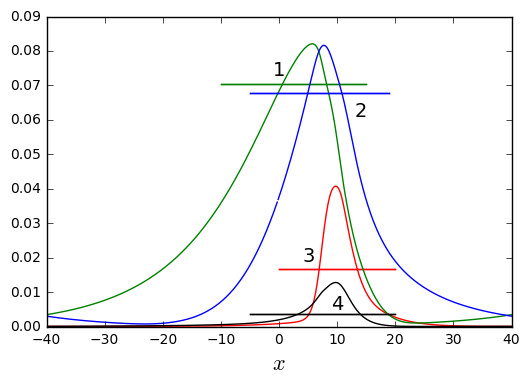
\includegraphics[width=0.5\linewidth]{pipetw_amp.png}}
\caption{Средние по сечению трубы амплитуды компонент движения бегущей волны (не зависят от $x$) и модельного порыва (функции $x$): 1 --- $\V_S$; 2 --- $\V_{2D}$ (отклонение от течения Пуазейля); 3 --- $\v_n$; 4 --- $\V_V$.}
\label{pipetw_amp_pic}
\end{figure}

Найденная бегущая волна повторяет качественные особенности модельного порыва, но количественно наблюдаются существенные отличия. Для сравнения на Рисунке \ref{pipetw_amp_pic} приведены средние по сечению трубы амплитуды компонент движения бегущей волны и модельного порыва. Для бегущей волны приведенные величины не зависят от продольной координаты. Графики для модельного порыва повторяют графики, приведенные на Рисунке~\ref{amp_pic}. По аналогии с модельным порывом, среднее течение $\V_\mathrm{tw}$ представлено в виде суммы двумерной $\V_\mathrm{2D,tw} = \overline{\V_\mathrm{tw}}^\theta$ и трехмерной  $\V_\mathrm{3D,tw} = \V_\mathrm{tw} - \V_\mathrm{2D,tw}$ составляющих. Трехмерная составляющая движения разложена на продольную $\V_\mathrm{S,tw}$ и поперечную $\V_\mathrm{V,tw}$ компоненты, ассоциированные с полосами и продольными вихрями, соответственно. Соотношения между интенсивностью различных компонент движения в бегущей волне сохраняется, но абсолютные значения оказываются значительно ниже. Наибольшее отличие наблюдается в интенсивности среднего поперечного движения $\V_\mathrm{V}$. В бегущей волне значение амплитуды этого движения почти в четыре раза ниже наибольшего значения, достигаемого в модельном порыве. Столь существенную разницу можно объяснить исходя из представлений о том, что решение на сепаратрисе является равновесным, и интенсивность продольных вихрей определяется необходимостью поддержания полос. В бегущей волне продольные вихри и полосы существует во всем течении. В модельном порыве протяженность продольных вихрей оказывается значительно ниже протяженности полос, соответственно для поддержания полос вихри в этом случае должны иметь большую интенсивность. 


\begin{figure}
\center{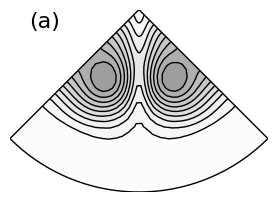
\includegraphics[width=0.33\linewidth]{pipetw_lin_amp.png} 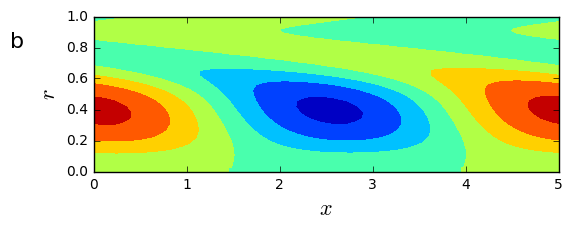
\includegraphics[width=0.6\linewidth]{pipetw_lin_ls.png}}
\caption{Наиболее быстро растущее собственное решение линейной задачи устойчивости поля скорости $\V_\mathrm{tw}$: (a) --- линии уровня амплитуды колебаний; (b) --- изолинии продольной компоненты скорости в сечении $\theta = 0$. Сплошные линии --- положительные значения, прерывистые --- отрицательные.}
\label{pipetw_lin_pic}
\end{figure}


Также, как в модельном порыве, пульсационная составляющая движения бегущей волны $\v_\mathrm{n,tw}$ возникает в результате линейной неустойчивости среднего течения $\V_\mathrm{tw}$. Наиболее быстрорастущее собственное решение линейной задачи устойчивости поля скорости $\V_\mathrm{tw}$ повторяет форму пульсационной составляющей движения и её фазовую скорость. Соответствующий инкремент нарастания $\lambda = 0.0085R/U$. Для сравнения с пульсационной составляющей движения $\v_\mathrm{n,tw}$, поле скорости которой представлено на Рисунке \ref{pipetw_pic}(c,d), на Рисунке \ref{pipetw_lin_pic}(a,b) приведены амплитуда колебаний наиболее быстро растущего решения линейной задачи устойчивости и его мгновенное поле скорости в продольном сечении трубы. Также, как для модельного порыва, для бегущей волны полученные в рамках линеаризованных уравнений пульсации имеют дополнительную симметрию отражения относительно сечения $\theta = \pi/4$, выражаемую уравнением \eqref{dop_sym_eq}. Пульсации достигают своего максимума между полосами повышенной и пониженной скорости. В этой области находится точка перегиба, если рассматривать среднее течение как функцию переменной~$\theta$. Вероятным механизмом образования пульсаций является механизм типа Кельвина-Гельмгольца.

%\lambda = - 0.0065

Получено решение уравнений Навье-Стокса в виде бегущей волны, описаны его основные свойства. Это решение воспроизводит основные элементы цикла поддержания модельного порыва, но имеет более простую форму. Поле скорости бегущей волны стационарно в сопутствующей системе отсчета. Осреднение вдоль трубы позволяет разделить его на среднюю и пульсационную составляющие. Показано, что пульсационная составляющая движения возникает в результате линейной неустойчивости среднего течения. Неустойчивость связана с наличием в среднем течении полос повышенной и пониженной скорости. Существование полос поддерживают стационарные продольные вихри. В следующих двух главах представлен механизм поддержания продольных вихрей, замыкающий цикл поддержания колебаний в этом решении. 


\section{Механизм поддержания продольных вихрей на примере решения в виде бегущей волны}

Принято считать, что продольные вихри, ответственные за образование полос в пристенных турбулентных течениях, возникают в результате некоторого нелинейного взаимодействия пульсаций, однако детали такого взаимодействия не были установлены. Прояснить процесс формирования продольных вихрей в рассматриваемых модельных течениях позволяет анализ уравнения, описывающего эволюцию продольной завихренности, полученного применением оператора ротора к уравнению Навье-Стокса \eqref{NS_eq}:
\begin{equation}\label{ox_eq}
\pd{\omega_x}{t} - \nu\nabla^2 \omega_x =  c_f \pd{\omega_x}{x} -  (\v \cdot \nabla) \omega_x + (\om \cdot \nabla) v_x.
\end{equation}
Здесь $\om = (\omega_x, \omega_r, \omega_\theta) = \rot \v$ --- вектор завихренности, $c_f$ --- скорость перемещения системы отсчета. Уравнение для средней составляющей продольной завихренности получается после осреднения \eqref{ox_eq} вдоль трубы и для решения в виде бегущей волны имеет вид:
\begin{equation}\label{OX_eq}
\pd{\Omega_x}{t} + (\V \cdot \nabla) \Omega_x - \nu\nabla^2 \Omega_x = - \overline{(\v' \cdot \nabla) \omega'_x}^x + \overline{ (\om' \cdot \nabla) v'_x }^x.
\end{equation}
Здесь  $\Om=(\Omega_x, \Omega_r, \Omega_\theta) = \overline{\om}^x$ и $\om'=(\omega'_x, \omega'_r, \omega'_\theta) = \om - \Om$ --- средняя и пульсационная составляющие вектора завихренности. Слагаемые в правой части уравнения \eqref{OX_eq} отвечают за генерацию $\Omega_x$, обусловленную нелинейным взаимодействием пульсаций. Второе и третье слагаемые в левой части уравнения отвечают за конвекцию существующей $\Omega_x$ и вязкие эффекты. Так как среднее течение во времени не меняется, источниковые слагаемые в правой части уравнения \eqref{OX_eq} компенсируются конвективным и вязким слагаемыми в левой его части. 

В скалярных переменных уравнение \eqref{OX_eq} имеет вид:
\begin{multline}\label{OX1_eq}
\pd{\Omega_x}{t} + V_r \pd{\Omega_x}{r} + \frac{V_\theta}{r} \pd{\Omega_x}{\theta}
 - \nu\left(\pd{^2\Omega_x}{r^2} + \frac{1}{r^2}\pd{^2\Omega_x}{\theta^2} + \frac{1}{r}\pd{\Omega_x}{r}\right)= \\
 - \overline{v'_x \pd{\omega'_x}{x}}^x - \overline{v'_r \pd{\omega'_x}{r}}^x - \overline{\frac{v'_\theta}{r} \pd{\omega'_x}{\theta}}^x
 + \overline{\omega'_x \pd{v'_x}{x}}^x + \overline{\omega'_r \pd{v'_x}{r}}^x + \overline{\frac{\omega'_\theta}{r} \pd{v'_x}{\theta}}^x.
\end{multline}
Для выявления определяющих механизмов генерации средней продольной завихренности удобнее рассмотреть уравнение эволюции квадрата $\Omega_x$, получающееся домножением всех членов \eqref{OX1_eq} на $2\Omega_x$. Положительный или отрицательный знак у полученных таким образом выражений в правой части уравнения показывает соответственно их положительный или отрицательный вклад в изменение $\Omega_x^2$, а, следовательно, и в интенсивность поперечного движения. Распределение $\Omega_x^2$ по сечению трубы представлено на Рисунке~\ref{OXgen_pic}(a). В большей части трубы средняя продольная завихренность близка к нулю. Области концентрации $\Omega_x$ находятся между полосами повышенной и пониженной скорости и соответствуют стационарным продольным вихрям (смотри Рисунок \ref{pipetw_pic}(b)). 

Анализ уравнения \eqref{OX1_eq} показал, что два слагаемых в правой части этого уравнения вносят определяющий вклад в производство средней продольной завихренности. Эти слагаемые имеют вид:
\begin{equation}\label{OXgen_terms}
- \overline{v'_x \frac{\d \omega'_x}{\d x}}^x + \overline{ \omega'_x \frac{\d v'_x}{\d x} }^x.
\end{equation}
Слагаемые \eqref{OXgen_terms} описывают нелинейное взаимодействие пульсаций продольной скорости $v'_x$ и пульсаций продольной завихренности $\omega'_x$. Между собой выделенные слагаемые равны в силу периодичности решения вдоль трубы. Слагаемые \eqref{OXgen_terms}, умноженные на $2\Omega_x$, представлены на Рисунке~\ref{OXgen_pic}(b), на Рисунке~\ref{OXgen_pic}(c) приведена сумма других слагаемых в правой части \eqref{OX_eq}, также умноженная на $2\Omega_x$. Вклад слагаемых \eqref{OXgen_terms} определяет форму поля $\Omega_x^2$ и более чем на порядок превосходит суммарный вклад других источниковых членов. Таким образом, нет сомнения в том, что стационарные продольные вихри возникают за счет действия выделенной пары слагаемых.

\begin{figure}
\center{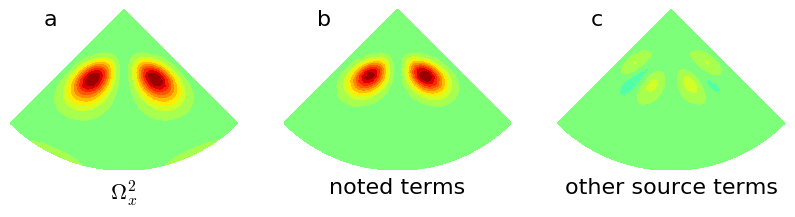
\includegraphics[width=1\linewidth]{pipetw_OXgen.png}}
\caption{Распределение по сечению трубы $\Omega_x^2$ (a) и вклад в генерацию $\Omega_x^2$ со стороны слагаемых, соответствующих слагаемым \eqref{OXgen_terms} (b) и другим слагаемым в правой части \eqref{OX_eq} (с). Изолинии построены с постоянным шагом, совпадающим для (b) и (c). Сплошные линии --- положительные значения, прерывистые --- отрицательные.}
\label{OXgen_pic}
\end{figure}

Отметим, что пульсации, соответствующие старшей собственной функции линейной задачи об устойчивости среднего стационарного течения, также демонстрируют приведенный выше механизм образования стационарных продольных вихрей. Важно, что это наблюдается только в том случае, когда при анализе устойчивости учитываются как продольная, так и поперечная составляющие среднего течения. Принято считать, что поперечное движение, определяя угловую неоднородность в распределении продольной скорости среднего течения, не может существенным образом влиять на свойства его устойчивости вследствие незначительности своей амплитуды. Поэтому при исследовании линейной устойчивости подобных течений, например, полосчатых структур в турбулентных потоках, наличие поперечного движения обычно не принимается во внимание. В нашем случае пренебрежение поперечным движением приводит к тому, что стационарное течение оказывается линейно устойчивым. Что еще более важно, наименее затухающее возмущение не воспроизводит при этом описанный механизм формирования продольных вихрей. Это связанно с тем, что форма пульсаций продольной завихренности $\omega'_x$ качественно меняется, хотя пульсации продольной скорости $v'_x$ сохраняют свою форму практически неизменной. Тем самым нарушается согласованность  $v'_x$ и $\omega'_x$, необходимая для обеспечения нужного вклада выражения \eqref{OXgen_terms} в производство продольной завихренности.

\begin{figure}
\center{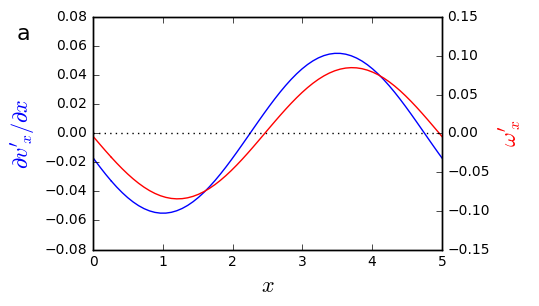
\includegraphics[width=0.5\linewidth]{pipetw_lin_cor.png}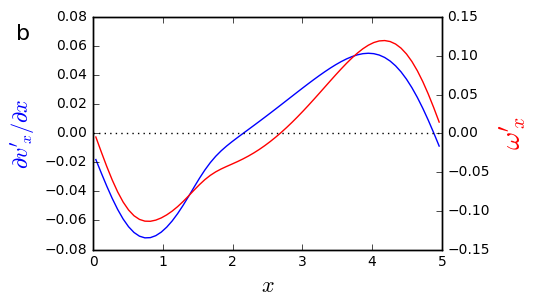
\includegraphics[width=0.5\linewidth]{pipetw_puls_cor.png}}
\caption{Значение $\d v_x' /\d x$ (кривая 1) и $\omega_x'$ (кривая 2) на прямой, проходящей через область, занятую положительным вихрем, при $r = 0.5, \theta = \pi/8$: (a) --- для пульсаций, полученных в линейном приближении; (b) --- для пульсационной составляющей движения бегущей волны. }
\label{OXgen_corr_pic}
\end{figure}

%Интересно отметить, что сумма слагаемых \eqref{OXgen_terms}, посчитанных для собственного решения линейной задачи устойчивости поля скорости $\V_\mathrm{tw}$, не зависит от $x$. 
%В линейном приближении слагаемые \eqref{OXgen_terms}, поддерживая существование продольных вихрей, сохраняют их независящими от продольной координаты. 
Анализ старшей собственной функции линейной задачи устойчивости позволяет в наиболее строгом виде продемонстрировать ряд важных свойств найденного механизма образования продольных вихрей. Так как среднее поле скорости $\V_\mathrm{tw}$ однородно вдоль трубы, возникающие на нем собственные возмущения меняются вдоль трубы по гармоническом закону. При фиксированных значениях $r$ и $\theta$ пусть  $v'_x = a \sin(\alpha x + \phi)$, $\omega_x' = b \sin(\alpha x + \psi)$, тогда слагаемые \eqref{OXgen_terms} будут иметь следующее значение:
\begin{equation*} \label{OXgen_iterms_1}
 - v'_x \frac{\d \omega'_x}{\d x} = - \alpha a b \sin(\alpha x + \phi) \cos(\alpha x + \psi),
\end{equation*}
\begin{equation*} \label{OXgen_iterms_2}
\omega'_x \frac{\d v'_x}{\d x} =  \alpha a b \cos(\alpha x + \phi) \sin(\alpha x + \psi),
\end{equation*}
\begin{equation} \label{OXgen_iterms_sum}
 - v'_x \frac{\d \omega'_x}{\d x} + \omega'_x \frac{\d v'_x}{\d x} = \alpha a b \sin(\psi - \phi).
\end{equation}
Интересно отметить, что сумма \eqref{OXgen_iterms_sum} не зависит от $x$, что, в частности, позволяет в последних трех выражениях упустить знак осреднения вдоль трубы. Эффективность производства  $\Omega_x$ определяется разностью фаз $\psi - \phi$. В области положительного вихря, при $a,b > 0$, наибольшее значение как первого, так и второго слагаемого достигается при $\psi - \phi = \pi/2$. В этом случае $\d \omega'_x/\d x$ и $v'_x$ положительно коррелированы, в то время как $\d v'_x/\d x$ и $\omega'_x$ --- отрицательно. В области отрицательного вихря ситуация меняется на противоположную. Расчет соответствующих коэффициентов корреляции показывает, что они близки к $\pm1$ в соответствующих областях. В качестве подтверждения на Рисунке \ref{OXgen_corr_pic}(a) представлены значения $\d v'_x/\d x$ и $\omega'_x$ на прямой, проходящей через область, занятую положительным вихрем, $r = 0.5, \theta = \pi/8$. Фазы выделенных компонент движения практически совпадают. Указанное свойство сохраняется для пульсационной составляющей движения $\v_\mathrm{n,tw}$, для которой аналогичные величины изображены на Рисунке \ref{OXgen_corr_pic}(b). Объяснить наблюдаемую согласованность фаз позволяет механизм образования пульсаций продольной завихренности, представленный в следующем разделе. 


\section{Механизм поддержания пульсаций продольной завихренности на примере решения в виде бегущей волны} \label{ox1gen_seq}

Объяснить согласованность фаз между пульсациями продольной скорости и пульсациями продольной завихренности, обеспечивающую поддержание продольных вихрей, позволяет анализ уравнения эволюции $\omega'_x$, полученного вычитанием \eqref{OX_eq} из \eqref{ox_eq}:
\begin{multline}\label{ox1_eq}
\pd{\omega'_x}{t} - c_f\pd{\omega'_x}{x} + (\V \cdot \nabla) \omega'_x - \nu \nabla^2 \omega'_x = - (\v' \cdot \nabla) \Omega_x
+(\Om \cdot \nabla) v'_x + \\ + (\om' \cdot \nabla) V_x - (\v' \cdot \nabla) \omega'_x  + (\om' \cdot \nabla) v'_x  + \overline{(\v' \cdot \nabla) \omega'_x}^x  - \overline{(\om' \cdot \nabla)v'_x}^x.
\end{multline}
В скалярных переменных уравнение \eqref{ox1_eq} имеет вид:
\begin{multline}\label{ox2_eq}
\pd{\omega'_x}{t} + (V_x - c_f)\pd{\omega'_x}{x} + V_r \pd{\omega_x'}{r} + \frac{V_\theta}{r} \pd{\omega'_x}{\theta} 
- \nu\nabla^2\omega'_x = \\
- v'_r \pd{\Omega_x}{r} - \frac{v'_\theta}{r} \pd{\Omega_x}{\theta} 
+ \Omega_x \pd{v'_x}{x} + \Omega_r \pd{v'_x}{r} + \frac{\Omega_\theta}{r} \pd{v'_x}{\theta}
+ \omega'_r \pd{V_x}{r} + \frac{\omega'_\theta}{r} \pd{V_x}{\theta} - \\ 
- v'_x \pd{\omega'_x}{x} - v'_r \pd{\omega'_x}{r} - \frac{v'_\theta}{r} \pd{\omega'_x}{\theta} 
+ \omega'_x \pd{v'_x}{x} + \omega'_r \pd{v'_x}{r} + \frac{\omega'_\theta}{r} \pd{v'_x}{\theta} + \\
+ \overline{v'_x \pd{\omega'_x}{x}}^x + \overline{v'_r \pd{\omega'_x}{r}}^x + \overline{\frac{v'_\theta}{r} \pd{\omega'_x}{\theta}}^x
- \overline{\omega'_x \pd{v'_x}{x}}^x - \overline{\omega'_r \pd{v'_x}{r}}^x - \overline{\frac{\omega'_\theta}{r} \pd{v'_x}{\theta}}^x.
\end{multline}
Работать удобнее с уравнением, описывающим изменение среднего квадрата пульсаций продольной завихренности $\overline{\omega'_x\omega'_x}^x$, получаемым умножением \eqref{ox2_eq} на~$2\omega'_x$ c последующим осреднением вдоль трубы. Слагаемые в этом уравнении не зависят от времени и продольной координаты. Сумма слагаемых в правой части уравнения компенсируется вязкими и конвективными членами в левой части. Как и в предыдущем случае, в правой части уравнения удается выделить слагаемые, ответственные за возникновение пульсаций~$\omega'_x$. 


Распределение $\overline{\omega'_x \omega'_x}^x$ по сечению трубы изображено на Рисунке~\ref{ox1gen_pic}(a). Основные пульсации $\omega'_x$ наблюдаются в центре расчетной области около оси трубы. На месте расположения продольных вихрей также присутствуют пульсации $\omega'_x$, но меньшей интенсивности. В остальной части трубы амплитуда пульсаций близка к нулю. Обнаружено, что за генерацию пульсаций $\omega'_x$ в центральной части трубы и на месте продольных вихрей отвечают два разных механизма. Первый дает пульсации большей амплитуды, однако, за возникновение стационарных продольных вихрей ответственны пульсации, производимые вторым механизмом, так как именно они оказываются согласованными с пульсациями $v'_x$ нужным образом.


\begin{figure}
\center{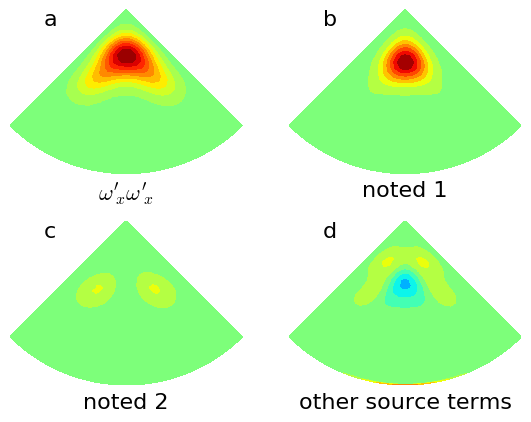
\includegraphics[width=0.66\linewidth]{pipetw_ox1gen.png}}
\caption{Распределение по сечению трубы среднего квадрата пульсаций продольной завихренности $\overline{\omega'_x \omega'_x }^x$ (а), вклад в производство $\overline{\omega'_x \omega'_x }^x$ со стороны слагаемых, соответствующих \eqref{ox1gen_add_terms} (b), \eqref{ox1gen_main_terms} (c) и сумме остальных слагаемых в правой части \eqref{ox2_eq} (d). Изолинии построены с постоянным шагом, совпадающим для (b)--(d). Сплошные линии --- положительные значения, прерывистые --- отрицательные, кривая 1 --- критический слой ($V_x = c_\mathrm{tw}$).}
\label{ox1gen_pic}
\end{figure}


Первый механизм формирования~$\omega'_x$ связан с наличием нормальных к стенке вихрей в пульсационной составляющей движения. Цепочка нормальных к стенке вихрей, чередующихся по знаку, двигается вниз по полосе пониженной скорости. Этим вихрям соответствуют области повышенной амплитуды пульсаций радиальной завихренности~$\omega'_r$. На Рисунке \ref{pipetw_or1_pic} приведено значение~$\omega'_r$ в сечении $r = 0.5$, нормальном к выделенной компоненте завихренности. Приведенные на \ref{pipetw_or1_pic}(a) значения посчитаны по пульсациям, полученным в рамках линеаризованных уравнений. Аналогичные значения для пульсационной составляющей движения $\v_{n,tw}$ представлены на Рисунке \ref{pipetw_or1_pic}(b). Амплитуда~$\omega'_x$ оказывается на порядок ниже амплитуды~$\omega'_r$, амплитуда~$\omega'_\theta$ в центральной части трубы равна нулю в силу симметрии. Таким образом, в центральной части трубы поле завихренности представлено в первую очередь радиальной компонентой и соответствует нормальным к стенке вихрям.

Пульсации продольной завихренности $\omega'_x$ возникают вследствие поворота нормальных к стенке вихрей, происходящего в присутствии градиента продольной скорости $\d V_x/ \d r$ между полосой замедления и осью трубы. Кроме того, наличие радиального градиента $\d V_x/ \d r$ связано с наличием угловой завихренности $\Omega_\theta = \d V_r / \d x - \d V_x / \d r$. Радиальная пульсационная завихренность $\omega'_r = \d v'_x / r \d \theta - \d v'_\theta / \d x$ за счет первого из слагаемых поворачивает стационарные угловые вихри так, что те также приобретают пульсационную продольную составляющую. В уравнении \eqref{ox1_eq} за описанный механизм отвечают слагаемые:
\begin{equation}\label{ox1gen_add_terms}
\frac{\d \omega'_x}{\d t} = \omega'_r \frac {\d V_x}{\d r} + \frac{\Omega_\theta}{r} \frac{\d v'_x}{\d \theta} + ...
\end{equation}
Несмотря на то, что выделенные в \eqref{ox1gen_add_terms} слагаемые имеют противоположные знаки и в значительной степени компенсируют друг друга при сложении, их вклад в производство $\omega'_x$ значителен (смотри Рисунок~\ref{ox1gen_pic}(b)). Они определяют форму пульсаций $\omega'_x$ в области между полосой замедления и осью трубы, где пульсации $\omega'_x$ достигают наибольшего значения. Эти пульсации, однако, практически не участвуют в образовании стационарной составляющей продольной завихренности. Это объясняется тем, что колебания $\omega'_x$, рождающиеся в результате описанного механизма, близки по фазе к колебаниям $v'_x$, так что каждое из слагаемых в выражении \eqref{OXgen_terms} при осреднении дает близкое к нулю значение.

\begin{figure}
\center{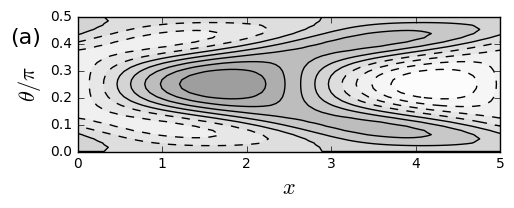
\includegraphics[width=0.45\linewidth]{pipetw_or1_lin.png} 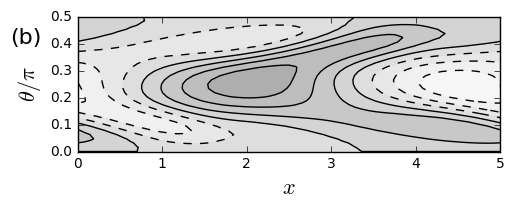
\includegraphics[width=0.45\linewidth]{pipetw_or1.png}}
\caption{Линии уровня нормальной к стенке компоненты завихренности $\omega_r'$ в сечении $r = 0.5$ для пульсаций, полученных в рамках линейного приближения (а) и для пульсационной составляющей движения бегущей волны (b). Сплошные линии --- положительные значения, прерывистые --- отрицательные.}
\label{pipetw_or1_pic}
\end{figure}

Второй механизм образования пульсаций продольной завихренности $\omega'_x$ связан с перераспределением уже существующей стационарной продольной завихренности $\Omega_x$ за счет пульсационной составляющей продольной скорости $v'_x$ (эффект сжатия/растяжения вихревых трубок). В уравнении \eqref{ox1_eq} за описываемый механизм отвечает слагаемое
\begin{equation}\label{ox1gen_main_terms}
\frac{\d \omega'_x}{\d t} = \Omega_x \frac {\d v'_x}{\d x} + ...
\end{equation}
Выделенное в \eqref{ox1gen_main_terms} слагаемое стремится произвести пульсации $\omega'_x$, пропорциональные $\d v'_x / \d x$, причем коэффициентом пропорциональности выступает средняя продольная завихренность. Соответственно,  механизм включается в областях концентрации~$\Omega_x$. В области расположения положительного вихря производимые пульсации $\omega'_x$ положительно пропорциональны пульсациям $\d v'_x / \d x$, а в области расположения отрицательного вихря --- отрицательно пропорциональны. Таким образом обеспечивается максимально возможная эффективность производства средней продольной завихренности нужного знака посредством второго из слагаемых \eqref{OXgen_terms}. Пульсации $-v'_x$ и $\d \omega'_x / \d x$ отказываются также согласованы нужным образом, и первое слагаемое \eqref{OXgen_terms} оказывается равно второму.

На Рисунке~\ref{ox1gen_pic}(c) приведен вклад выделенного в \eqref{ox1gen_main_terms} слагаемого в производство $\overline{\omega'_x \omega'_x}^x$. Это слагаемое определяет форму пульсаций в области существования продольных вихрей --- между полосами повышенной и пониженной скорости. Суммарный вклад других слагаемых в правой части \eqref{ox1_eq}, не попавших на Рисунки~\ref{ox1gen_pic}(b,c), изображен на Рисунке~\ref{ox1gen_pic}(d). Эти слагаемые также поддерживают существование колебаний в области расположения продольных вихрей, но их влияние оказывается значительно ниже влияния выделенного в \eqref{ox1gen_main_terms} слагаемого. В точке, где $\Omega_x$ достигает максимума, приведенная на Рисунке (d) величина оказывается в три раза ниже приведенной на Рисунке (c). Стоит также учитывать, что пульсации, генерируемые слагаемыми, которым соответствует Рисунок (d), не обязательно согласованы по фазе с пульсациями продольной скорости нужным для поддержания продольных вихрей образом, так что роль слагаемых (d) в поддержании продольных вихрей может оказаться еще ниже. 

Отметим, что выполнено необходимое условие для образования пульсаций $\omega'_x$ слагаемым \eqref{ox1gen_main_terms}. Продольные вихри образуются вблизи критического слоя, в котором средняя скорость жидкости совпадает с фазовой скоростью бегущей волны $c_\mathrm{tw} = 0.77$. Критическому слою соответствует кривая 1 на Рисунке \ref{ox1gen_pic}(c). По этой причине в системе отчета бегущей волны в области образования продольных вихрей все конвективные слагаемые в правой части \eqref{ox2_eq} близки к нулю. В отсутствии конвекции производимые слагаемым \eqref{ox1gen_main_terms} пульсации $\omega'_x$ сохраняют согласованность фаз с пульсациями $\partial v'_x / \partial x$, что необходимо для дальнейшего роста амплитуды пульсаций $\omega'_x$ и формирования стационарных продольных вихрей. 

Таким образом, продольные вихри образуются в области возбуждения пульсаций, между полосами повышенной и пониженной скорости, так как именно в этой области средняя скорость жидкости совпадает с фазовой скоростью пульсаций и пульсации имеют наибольшую амплитуду. Пульсации продольной скорости сжимая и растягивая существующие в потоке вихревые трубки формируют пульсации продольной завихренности, согласованные с пульсациями продольной скорости таким образом, что их нелинейное взаимодействие поддерживает продольны вихри. Образуясь между соседними полосами повышенной и пониженной скорости, продольные вихри оказываются расположены наиболее удачным образом для поддержания существования этих полос. 

Описанный механизм генерации пульсаций продольной завихренности объясняет необходимость учета поперечного движения при исследовании устойчивости стационарного течения. Пренебрежение связанной с поперечным движением $\Omega_x$ делает невозможным генерацию $\omega'_x$ в форме, необходимой для сохранения поперечного движения, а следовательно и всего процесса самоподдержания пульсаций.


\section{Механизм поддержания продольных вихрей и пульсаций продольной завихренности в модельном порыве} \label{edge_oxgen}

В работе выделен механизм поддержания продольных вихрей в модельном порыве. Это механизм аналогичен механизму, поддерживающему продольные вихри в решении, имеющем вид бегущей волны. При изучении решения, имеющего вид бегущей волны, разделение на среднюю и пульсационную составляющие движения выполняется осреднением вдоль трубы. При изучении модельного порыва осреднение выполняется по времени в сопутствующей системе отсчета. Пусть $\V_\mathrm{mp} = (V_x, V_r, V_\theta) = \overline{\v_\mathrm{mp}}^t$ и $\v'_\mathrm{mp} = (v'_x, v'_r, v'_\theta) = (\v_\mathrm{mp} - \V_\mathrm{mp}$) --- средняя и пульсационная составляющие поля скорости модельного порыва $\v_\mathrm{mp} = (v_x, v_r, v_\theta)$, а $\Om_\mathrm{mp} = (\Omega_x, \Omega_r, \Omega_\theta) = \rot \V_\mathrm{mp}$ и $\om'_\mathrm{mp} = (\omega'_x, \omega'_r, \omega'_\theta) = \rot \v'_\mathrm{mp}$ --- средняя и пульсационная составляющие поля завихренности $\om_\mathrm{mp} = (\omega_x, \omega_r, \omega_\theta) = \rot \v_\mathrm{mp}$ (<<mp>> --- <<model puff>>). 

Так же, как в бегущей волне, в модельном порыве существуют стационарные продольные  вихри, поддерживающие существование полос, но в этом случае они имеют ограниченную протяженность (смотри Рисунок \ref{VEL_cs_pic}). Установить механизм образования стационарных продольных вихрей в модельном порыве позволяет анализ уравнения баланса стационарной продольной завихренности, полученного осреднением по времени в системе отсчета порыва уравнения эволюции продольной завихренности \eqref{ox_eq}: 
\begin{equation} \label{time_OX_eq}
\pd{\Omega_x}{t} - c_\mathrm{mp} \pd{\Omega_x}{x} + (\V \cdot \nabla) \Omega_x - \nu\nabla^2 \Omega_x = (\Om \cdot \nabla) V_x - \overline{(\v' \cdot \nabla) \omega'_x}^t + \overline{(\om' \cdot \nabla) v'_x}^t.
\end{equation}
Здесь $c_\mathrm{mp}$ --- скорость перемещения модельного порыва. В правой части \eqref{time_OX_eq} собраны слагаемые--источники $\Omega_x$. Первое из них описывает образование $\Omega_x$ за счет сжатия, растяжения и поворота существующих в среднем течении вихрей. Второе и третье описывают нелинейное взаимодействие пульсаций. Так как $\Omega_x$ во времени не меняется, производство $\Omega_x$ слагаемыми из правой части уравнения компенсируется конвективным и вязким слагаемыми в левой его части. 

В скалярных переменных уравнение \eqref{time_OX_eq} имеет вид:
\begin{multline}\label{time_OX1_eq}
\pd{\Omega_x}{t} + (V_x - c_\mathrm{mp})\pd{\Omega_x}{x} + V_r \pd{\Omega_x}{r} + \frac{V_\theta}{r} \pd{\Omega_x}{\theta} - \nu\nabla^2\Omega_x= \Omega_x \pd{V_x}{x} + \Omega_r \pd{V_x}{r} + \\ + \frac{\Omega_\theta}{r} \pd{V_x}{\theta}
 - \overline{v'_x \pd{\omega'_x}{x}}^t - \overline{v'_r \pd{\omega'_x}{r}}^t - \overline{\frac{v'_\theta}{r} \pd{\omega'_x}{\theta}}^t
 + \overline{\omega'_x \pd{v'_x}{x}}^t + \overline{\omega'_r \pd{v'_x}{r}}^t + \overline{\frac{\omega'_\theta}{r} \pd{v'_x}{\theta}}^t.
\end{multline}
Работать удобнее с уравнением баланса квадрата стационарной продольной завихренности $\Omega_x^2$, полученным скалярным умножением \eqref{time_OX_eq} на $2\Omega_x$. Положительное или отрицательное значение источниковых членов в этом уравнении говорит о положительном или отрицательном их влиянии на образование~$\Omega_x$. 


\begin{figure}[h]
\center{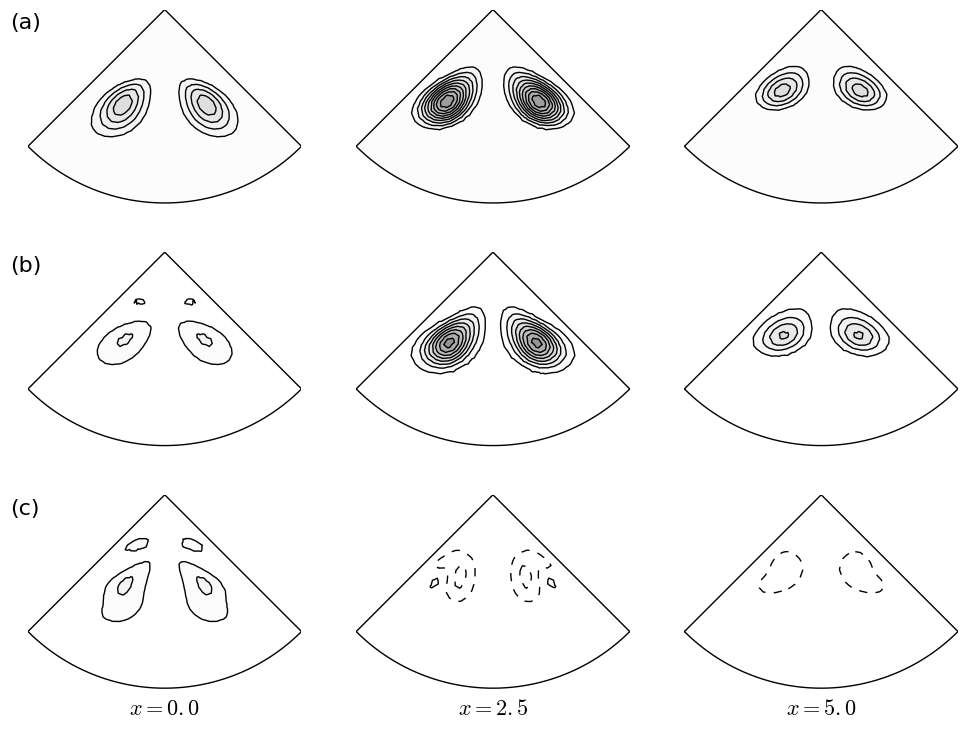
\includegraphics[width=1\linewidth]{puff_OXgen.png}}
\caption{В нескольких сечения трубы приведены значения $\Omega_x^2$ (ряд (а)) и вклада в образование $\Omega_x^2$ со стороны слагаемых, соответствующих слагаемым \eqref{time_OXgen_terms} (ряд (b)) и другим слагаемым в правой части уравнения \eqref{time_OX_eq} (ряд (c)). Представлено три сечения из области существования продольных вихрей, $x=0,2.5,5$. Изолинии построены с постоянным шагом, совпадающим для каждого ряда и между рядами (b) и (c). Сплошные линии --- положительные значения, прерывистые --- отрицательные.}
\label{mp_OXgen_pic}
\end{figure}

Анализ уравнения \eqref{time_OX_eq} позволил установить механизм поддержания стационарных продольных вихрей, аналогичный выделенному при изучении бегущей волны. За поддержание стационарных продольных вихрей отвечают слагаемые 
\begin{equation} \label{time_OXgen_terms}
- \overline{v'_x \pd{\omega'_x}{x}}^t + \overline{\omega'_x \pd{v'_x}{x}}^t. 
\end{equation}
На Рисунке \ref{mp_OXgen_pic} в ряду (а) приведено значение $\Omega_x^2$ в трех сечениях трубы из области, где продольные вихри имеют существенную амплитуду. Распределение стационарной продольной завихренности соответствует наличию стационарных продольных вихрей. На Рисунке \ref{mp_OXgen_pic} в рядах (b) и (с) в тех же сечения приведены значение слагаемых \eqref{time_OXgen_terms}, умноженных на $2\Omega_x$, и значение других слагаемых в правой части уравнения \eqref{time_OX_eq}, также умноженных на $2\Omega_x$. Вклад слагаемых \eqref{time_OXgen_terms} в генерацию $\Omega_x^2$ значительно превосходит вклад других источниковых членов и определяют форму поля стационарной продольной завихренности. 

\begin{figure}[h]
\center{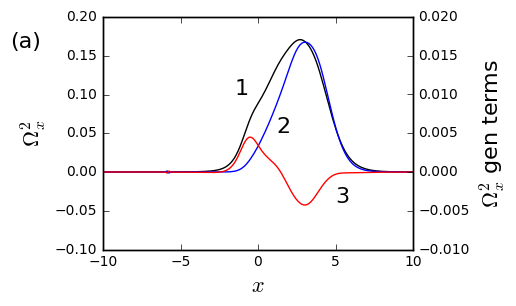
\includegraphics[width=0.5\linewidth]{xline_OXgen.png}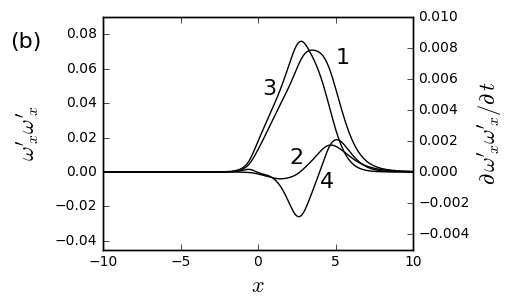
\includegraphics[width=0.5\linewidth]{xline_ox1gen.png}}
\caption{На прямой, проходящей через область, занятую продольным вихрем, при $r = 0.5, \theta = \pi/8$, приведены: (a) --- квадрат стационарной продольной завихренности (кривая 1), вклад в его производство со стороны \eqref{time_OXgen_terms} (кривая  2) и других слагаемых в правой части уравнения \eqref{time_OX_eq} (кривая 3); (b) --- средний квадрат пульсаций продольной завихренности $\overline{\omega'_x \omega'_x}^t$ (кривая 1) и вклад в его производство со стороны \eqref{time_ox1gen_terms1} (кривая  2), \eqref{time_ox1gen_term2} (кривая  3) и других слагаемых в правой части уравнения \eqref{time_ox1_eq} (кривая  4).}
\label{xline_oxgen_pic}
\end{figure}

На Рисунке \ref{xline_oxgen_pic}(a) приведено значение $\Omega_x^2$ (кривая 1) и ответственных за его генерацию слагаемых на прямой, проходящей через область, занятую продольным вихрем, при $r = 0.5, \theta = \pi/8$. Из этих графиков также видно, что хотя существует небольшой участок вблизи $x=0$, на котором слагаемые \eqref{time_OXgen_terms} (кривая 2) уступают другим источниковым слагаемым (кривая 3), именно эти слагаемые дают подавляющий вклад в образование стационарной продольной завихренности. Таким образом, нет сомнения, что за генерацию стационарных продольных вихрей ответственны слагаемые \eqref{time_OXgen_terms}. 

В модельном порыве, слагаемые \eqref{time_OXgen_terms} имеют близкие значения (смотри Рисунок \ref{OXgen_terms_cmp_pic}), так как поле скорости модельного порыва в области существования продольных вихрей близко к полю скорости бегущей волны. В модельном порыве сохраняется отмеченная в предыдущем разделе согласованность фаз между пульсациями продольной скорости $v'_x$ и пульсациями продольной завихренности $\omega'_x$, однако форма пульсационной составляющей движения оказывается несколько более сложной. Согласованность фаз объясняется механизмом образования пульсаций продольной завихренности $\omega'_x$, выделенным в модельном порыве, который также аналогичен механизму, найденному в бегущей волне. 


\begin{figure}[h]
\center{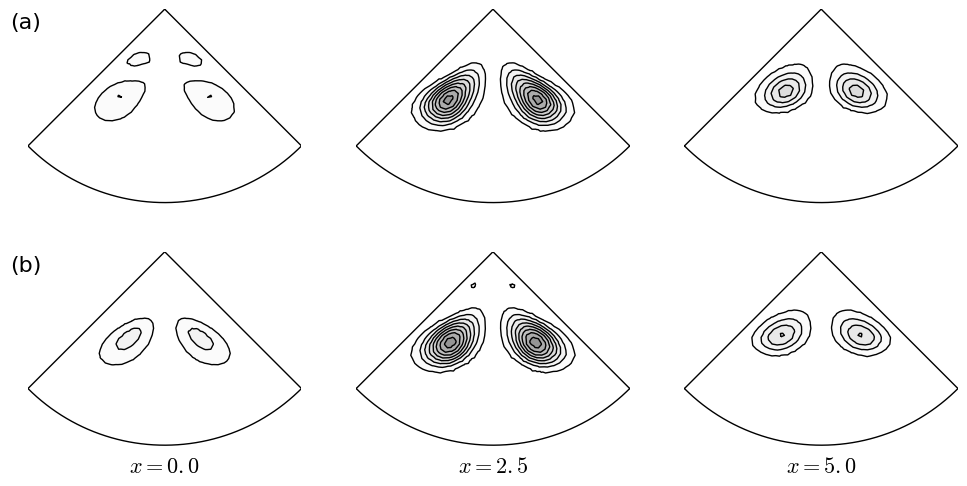
\includegraphics[width=1\linewidth]{OXgen_terms_cmp.png}}
\caption{Значение первого (ряд (а)) и второго (ряд (b)) слагаемых \eqref{time_OXgen_terms} в сечениях трубы $x=0,2.5,5$. }
\label{OXgen_terms_cmp_pic}
\end{figure}


Выделить механизм образования пульсаций продольной завихренности $\omega'_x$ позволяет анализ уравнения, полученного вычитанием \eqref{time_OX_eq} из \eqref{ox_eq}, описывающего эволюцию $\omega'_x$:
\begin{multline}\label{time_ox1_eq}
\pd{\omega'_x}{t} - c_\mathrm{tw}\pd{\omega'_x}{x} + (\V \cdot \nabla) \omega'_x - \nu \nabla^2 \omega'_x = - (\v' \cdot \nabla) \Omega_x +(\Om \cdot \nabla) v'_x + \\ + (\om' \cdot \nabla) V_x - (\v' \cdot \nabla) \omega'_x  + (\om' \cdot \nabla) v'_x  + \overline{(\v' \cdot \nabla) \omega'_x}^t  - \overline{(\om' \cdot \nabla)v'_x}^t.
\end{multline}
Это уравнение записано в системе отсчета, перемещающейся со скоростью $c_\mathrm{tw}$ бегущей волны, соответствующей пульсационной составляющей движения (осреднение по времени выполняется в системе отсчета порыва). Из анализа пульсационной составляющей движения значение $c_\mathrm{tw}$ выбрано равным $0.77U$. 
В скалярных переменных уравнение \eqref{time_ox1_eq} имеет вид:
\begin{multline}\label{time_ox2_eq}
\pd{\omega'_x}{t} + (V_x - c_\mathrm{tw})\pd{\omega'_x}{x} + V_r \pd{\omega_x'}{r} + \frac{V_\theta}{r} \pd{\omega'_x}{\theta} 
- \nu\nabla^2\omega'_x = - v'_x \pd{\Omega_x}{x} - v'_r \pd{\Omega_x}{r} - \\ - \frac{v'_\theta}{r} \pd{\Omega_x}{\theta} 
+ \Omega_x \pd{v'_x}{x} + \Omega_r \pd{v'_x}{r} + \frac{\Omega_\theta}{r} \pd{v'_x}{\theta}
+ \omega'_x \pd{V_x}{x} + \omega'_r \pd{V_x}{r} + \frac{\omega'_\theta}{r} \pd{V_x}{\theta} - \\ 
- v'_x \pd{\omega'_x}{x} - v'_r \pd{\omega'_x}{r} - \frac{v'_\theta}{r} \pd{\omega'_x}{\theta} 
+ \omega'_x \pd{v'_x}{x} + \omega'_r \pd{v'_x}{r} + \frac{\omega'_\theta}{r} \pd{v'_x}{\theta} + \\
+ \overline{v'_x \pd{\omega'_x}{x}}^t + \overline{v'_r \pd{\omega'_x}{r}}^t + \overline{\frac{v'_\theta}{r} \pd{\omega'_x}{\theta}}^t
- \overline{\omega'_x \pd{v'_x}{x}}^t - \overline{\omega'_r \pd{v'_x}{r}}^t - \overline{\frac{\omega'_\theta}{r} \pd{v'_x}{\theta}}^t.
\end{multline}
Работать удобнее с уравнением баланса пульсаций продольной завихренности $\overline{\omega'_x \omega'_x}^t$, полученным скалярным умножением \eqref{time_ox2_eq} на~$2 \omega'_x$ с последующим осреднением по времени. Анализ этого уравнения позволил выделить две группы слагаемых, ответственных за образование пульсаций продольной завихренности, имеющих вид:
\begin{equation}\label{time_ox1gen_terms1}
\frac{\d \omega'_x}{\d t} = \omega'_r \frac {\d V_x}{\d r} + \frac{\Omega_\theta}{r} \frac{\d v'_x}{\d \theta} + 
\end{equation}
\begin{equation}\label{time_ox1gen_term2}
+\Omega_x \frac {\d v'_x}{\d x} + ...
\end{equation}


\begin{figure}[h!]
\center{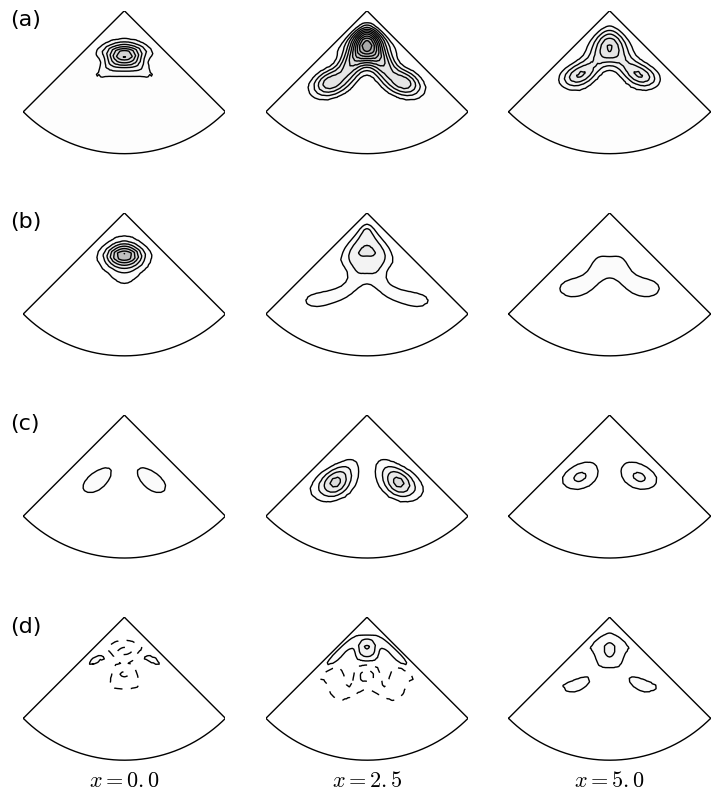
\includegraphics[width=0.9\linewidth]{puff_ox1gen.png}}
\caption{В нескольких сечения трубы приведена интенсивность пульсаций продольной завихренности $\overline{\omega'_x \omega'_x}^t$ (ряд а) и вклад в генерацию $\overline{\omega'_x \omega'_x}^t$ со стороны слагаемых, соответствующих слагаемым \eqref{time_ox1gen_terms1} (ряд b), слагаемому \eqref{time_ox1gen_term2} (ряд с) и другим слагаемым в правой части \eqref{time_ox1_eq} (ряд d). Изолинии построены с постоянным шагом, совпадающим внутри каждого ряда и между рядами (b)--(d). Сплошные линии --- положительные значения, прерывистые --- отрицательные.}
\label{mp_ox1gen_pic}
\end{figure}


На Рисунке \ref{mp_ox1gen_pic} в нескольких сечениях трубы приведены амплитуда пульсаций продольной завихренности $\overline{\omega'_x \omega'_x}^t$ (ряд (а)) и вклада в её поддержание со стороны слагаемых \eqref{time_ox1gen_terms1} (ряд (b)), слагаемых \eqref{time_ox1gen_term2} (ряд (с)) и слагаемых в правой части уравнения \eqref{time_ox2_eq}, не вошедших в \eqref{time_ox1gen_terms1} и \eqref{time_ox1gen_term2}, (ряд (d)). (Для того, чтобы вычислить вклад слагаемых уравнения \eqref{time_ox2_eq} в генерацию $\overline{\omega'_x \omega'_x}^t$, их значение умножено на $2\omega'_x$ с последующим осреднением по времени.) Слагаемые \eqref{time_ox1gen_terms1} отвечают за поворот нормальных к стенке вихрей, присутствующих в пульсационной составляющей движения. Приобретая продольную составляющую, эти вихри обеспечивают формирование значительных по амплитуде пульсаций $\omega'_x$ в области между полосой замедления и осью трубы. Однако на месте продольных вихрей эти слагаемые на $\omega'_x$ существенного влияния не оказывают. Кроме того, пульсации $\omega'_x$, создаваемые слагаемыми \eqref{time_ox1gen_terms1}, согласованны с пульсациями $v'_x$ таким образом, что не могут участвовать в поддержании $\Omega_x$. За образование пульсаций $\omega'_x$ на месте продольных вихрей ответственно слагаемое \eqref{time_ox1gen_term2}. Это слагаемое создает пульсации $\omega'_x$, согласованные с пульсациями $v'_x$ так, что их нелинейное взаимодействие эффективно поддерживает существование продольных вихрей. Другие слагаемые в правой части уравнения \eqref{time_ox2_eq} на месте продольных вихрей существенного влияния на $\omega'_x$ не оказывают. 


На Рисунке \ref{xline_oxgen_pic} приведена интенсивность пульсаций продольной завихренности $\overline{\omega'_x \omega'_x}^t$ (кривая 1) и вклад в её поддержание со стороны различных слагаемых уравнения \eqref{time_ox2_eq} на прямой, проходящей через область, занятую продольным вихрем, $r = 0.5, \theta = \pi/8$. Как только что обсуждалось, подавляющий вклад в генерацию $\overline{\omega'_x \omega'_x}^t$ дает слагаемое \eqref{time_ox1gen_term2} (кривая~3). Это слагаемое определяет интенсивность пульсаций $\omega'_x$ в области, занятой продольными вихрями. Другие слагаемые в правой части уравнения (кривые 2, 4) имеют значительно меньшее влияние. Таким образом может быть сделан вывод о том, что за образование пульсаций $\omega'_x$, участвующих в поддержании стационарных продольных вихрей, ответственно слагаемое \eqref{time_ox1gen_term2}. Это слагаемое отвечает за сжатие и растяжение существующих в стационарном течении вихревых нитей и обеспечивает необходимую для поддержания стационарных продольных вихрей согласованность фаз между $\omega'_x$ и $v'_x$ (смотри детали в предыдущем разделе). 

Выделен механизм поддержания стационарных продольных вихрей в модельном порыве. Выделенный механизм аналогичен механизму поддержания продольных вихрей в решении, имеющем вид бегущей волны. Сжимая и растягивая существующие вихревые нити, соответствующие стационарным продольным вихрям, пульсации продольной скорости формируют пульсации продольной завихренности, согласованные с пульсациями продольной скорости таким образом, что их нелинейное взаимодействие поддерживает существование продольных вихрей. 


\section{Выводы по главе}

В предыдущей главе представлены результаты численного исследования модельного порыва, в котором было составлено представление о его внутренней структуре и механизме поддержания колебаний. В подвижной системе отсчета в модельном порыве выделяются стационарные полосы повышенной и пониженной скорости, вытянутые вдоль стенки трубы. Полосы образуются под действием стационарных продольных вихрей, которые формируются в результате нелинейного взаимодействия нестационарных пульсаций, возникающих из-за неустойчивости полосчатого движения. В настоящей главе представлены определяющие элементы нелинейного механизма образования продольных вихрей. Таким образом, определены все элементы цикла самоподдержания колебаний внутри модельного порыва. 

Установлено, что пульсации продольной скорости формируют пульсации продольной завихренности сжимая и растягивая существующие вихревые нити, соответствующие стационарным продольным вихрям. Возникающие пульсации продольной скорости и пульсации продольной завихренности оказываются согласованными таким образом, что их нелинейное взаимодействие поддерживает продольные вихри. Таким образом продольные вихри формируются на месте возникновения пульсаций, между полосами повышенной и пониженной скорости, оказываясь расположенными наиболее удачным образом для поддержания существования этих полос.

Пульсации возникают в результате линейной неустойчивости полосчатого течения и могут быть воспроизведены в рамках линеаризованных уравнений. Решения линейной задачи устойчивости также воспроизводят описанный выше механизм поддержания продольных вихрей, но только в том случае, когда в исследуемом на устойчивость течении учтено не только продольное, но и поперечное движение, соответствующее наличию продольных вихрей. Несмотря на небольшую амплитуду поперечного движения, его учет необходим для адекватного описания пульсаций продольной завихренности. 

Также в главе приведены результаты исследования решения в виде бегущей волны. Это решение является предельным состоянием решения, эволюционирующего на сепаратрисе, найденного в непротяженной расчетной области. Поле скорости этого решения напоминает поле скорости модельного порыва в области существенной амплитуды пульсаций. Оба решения воспроизводит общий механизм самоподдержания. Анализ решения в виде бегущей волны позволил в более простой и в тоже время строгой форме продемонстрировать особенности движения, обеспечивающие работу выделенного механизма поддержания продольных вихрей. 

Указания на существенную роль слагаемых \eqref{time_OXgen_terms} в процессе поддержания продольных вихрей можно найти в работах \cite{Hamilton1995, Schoppa2002}. Работ, в которых был бы описан механизм формирования пульсаций продольной завихренности, объясняющий существенное отличие слагаемого \eqref{time_OXgen_terms} от нуля, нам не известно. Выделенный механизм образования продольных вихрей имеет характер неустойчивости. Скорость роста пульсаций продольной завихренности пропорциональна интенсивности продольных вихрей, в то время, как скорость роста интенсивности продольных вихрей пропорциональна амплитуде пульсаций продольной завихренности. Представления о том, что продольные вихри могут возникать в результате неустойчивости неоднородного вдоль трубы поля скорости, развиваются в асимптотических моделях в \cite{Craik1977, Hall2010}. Неустойчивость такого рода называют неустойчивость Крейка--Лейбовича второго типа. 


